\section{Laparoscopic tool manipulation}

\subsection{Tool pose}

\begin{center}
\begin{figure}[H]
\centering
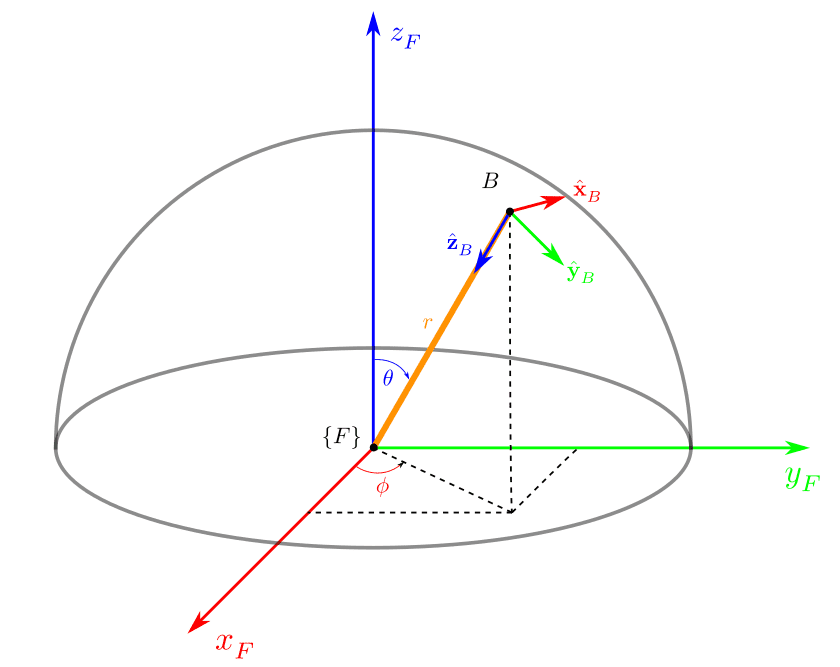
\includegraphics[width=12cm]{images/fulcrum-space.png}\\
\caption{Tool pose at target point $B$ calculated with respect to Fulcrum's reference frame $\lbrace F \rbrace$}
\end{figure}
\end{center}

The laparoscopic tool pose is given by the position and orientation vectors at target point $B$ with respect to the coordinate frame $\lbrace F \rbrace$.
The pose is given by the following transformation matrix
\[
{}^{F}T_B = \begin{bmatrix}
{}^{F}R_B & {}^{F}\mathbf{p}^{}_B \\
\mathbf{0} & 1 \\
\end{bmatrix}
\;\; where \;\;
{}^{F}R_B = \begin{bmatrix}
\hat{\mathbf{x}}^{}_B & \hat{\mathbf{y}}^{}_B & \hat{\mathbf{z}}^{}_B \\
\end{bmatrix}
\]

\[
\hat{\mathbf{x}}^{}_B = \hat{\mathbf{θ}} = cos(θ)cos(φ)\hat{\mathbf{x}}^{}_F + cos(θ)sin(φ)\hat{\mathbf{y}}^{}_F - sin(θ)\hat{\mathbf{z}}^{}_F
= \begin{bmatrix}
cos(θ)cos(φ) \\
cos(θ)sin(φ) \\
- sin(θ) \\
\end{bmatrix}
\]

\[
\hat{\mathbf{y}}^{}_B = \hat{\mathbf{φ}} = -sin(φ)\hat{\mathbf{x}}^{}_F + cos(φ)\hat{\mathbf{y}}^{}_F
= \begin{bmatrix}
-sin(φ) \\
cos(φ) \\
0 \\
\end{bmatrix}
\]

\[
\hat{\mathbf{z}}^{}_B = - \hat{\mathbf{r}} = - (sin(θ)cos(φ)\hat{\mathbf{x}}^{}_F + sin(θ)sin(φ)\hat{\mathbf{y}}^{}_F + cos(θ)\hat{\mathbf{z}}^{}_F)
= \begin{bmatrix}
-sin(θ)cos(φ) \\
-sin(θ)sin(φ) \\
-cos(θ) \\
\end{bmatrix}
\]

The position of the point $B$ is given in spherical coordinates by:
\begin{itemize}
	\item $r=ρ$ : outside penetration of laparoscopic tool
	\item $θ=β$ : altitude angle
	\item $φ=α$ : orientation angle
\end{itemize}
thus the position with respect to the coordinate frame $\lbrace F \rbrace$ is given by
\[
{}^{F}\mathbf{p}^{}_B = \begin{bmatrix}
ρsin(β)cos(α) \\
ρsin(β)sin(α) \\
ρcos(β) \\
\end{bmatrix} = ρ \hat{\mathbf{r}}
\]

The above goal point must be the same as the $TCP$ point of the robot's end-effector. This means, that this pose must be converted with respect to the robot's reference frames.
\[
{}^{U}T^{}_{TCP} = {}^{U}T^{}_{B}
\]
\[
{}^{U}T^{}_{0} \; {}^{0}T^{}_{7} \; {}^{7}T^{}_{TCP} = {}^{U}T^{}_{F} \; {}^{F}T^{}_{B}
\]
\begin{equation}
{}^{0}T^{}_{7} = {}^{U}T^{-1}_{0} \; {}^{U}T^{}_{F} \; {}^{F}T^{}_{B} \; {}^{7}T^{-1}_{TCP}
\end{equation}

\subsection{Pivoting motion with respect to Fulcrum Point}

\subsubsection{Circular trajectory of tool tip}

\begin{center}
\begin{figure}[H]
\centering
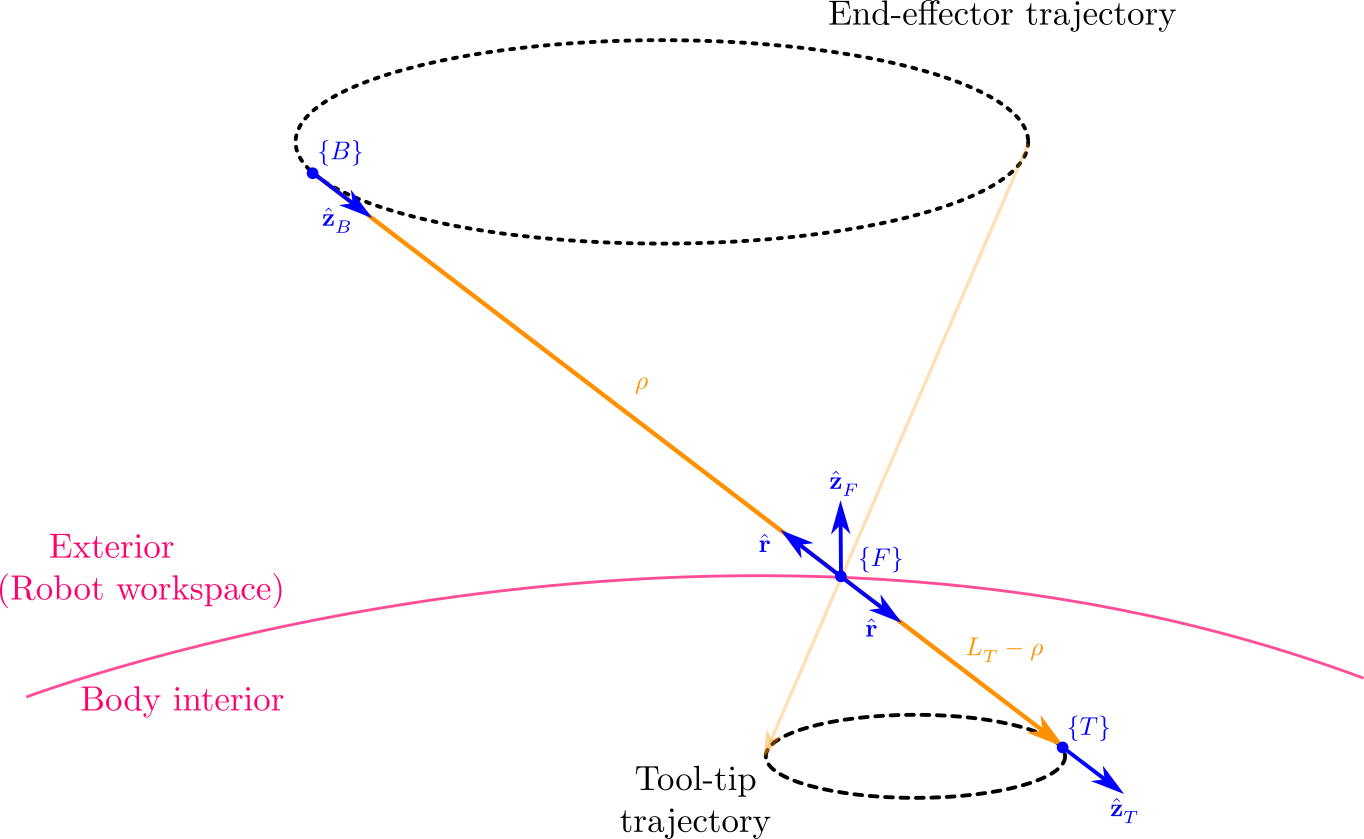
\includegraphics[width=12cm]{images/circular-trajectory-wrt-fulcrum.png}\\
\caption{Circular trajectory of tool tip with respect to Fulcrum reference frame}
\end{figure}
\end{center}

To generate a circular trajectory for the pivot movement we must specify the center of the circle 
and a vector whose magnitude is the radius of the circle and it’s direction gives the orientation 
of the plane that the circle lies at. The simplest case of a circular trajectory is the one, 
whose circle lies in a plane parallel to the xy plane.


We first consider the motion of the laparoscopic tool tip on a circle parallel to a z-plane, with respect to the $\lbrace F \rbrace$ coordinate frame.
\[
(x^{}_{F} - x^{}_{F0})^2 + (y^{}_{F} - y^{}_{F0})^2 = r_0^2, \;\; z^{}_{F} = z^{}_{F0}
\]
It's often more convenient to express trajectories in a parametric form, which makes it easier to calculate all the waypoints of the trajectory
\[
\begin{cases}
x^{}_{F} = r_0cos(2πt) + x^{}_{F0} \\
y^{}_{F} = r_0sin(2πt) + y^{}_{F0} \\
z^{}_{F} = z^{}_{F0}
\end{cases} ,
\;\;
t \in [0, 1]
\]
After having calculated the cartesian coordinates we can calculate the spherical coordinates as follows
\begin{equation}
\label{eqns:cartesian-to-spherical}
\begin{cases}
r = \sqrt{x^{2}_{F} + y^{2}_{F} + z^{2}_{F}} \\
θ = atan2 \left( \sqrt{x^{2}_{F} + y^{2}_{F}}, z^{}_{F} \right) \\
φ = atan2(y^{}_{F}, x^{}_{F})
\end{cases}
\end{equation}

\subsubsection{Circular arc trajectory of tool tip}

To generate a circular arc trajectory for a pivot motion we must specify the same parameters as 
in the circular trajectory as well as the length of the arc or the total angle of the arc 
section.


\subsubsection{Line segment trajectory of tool tip}

\begin{center}
\begin{figure}[H]
\centering
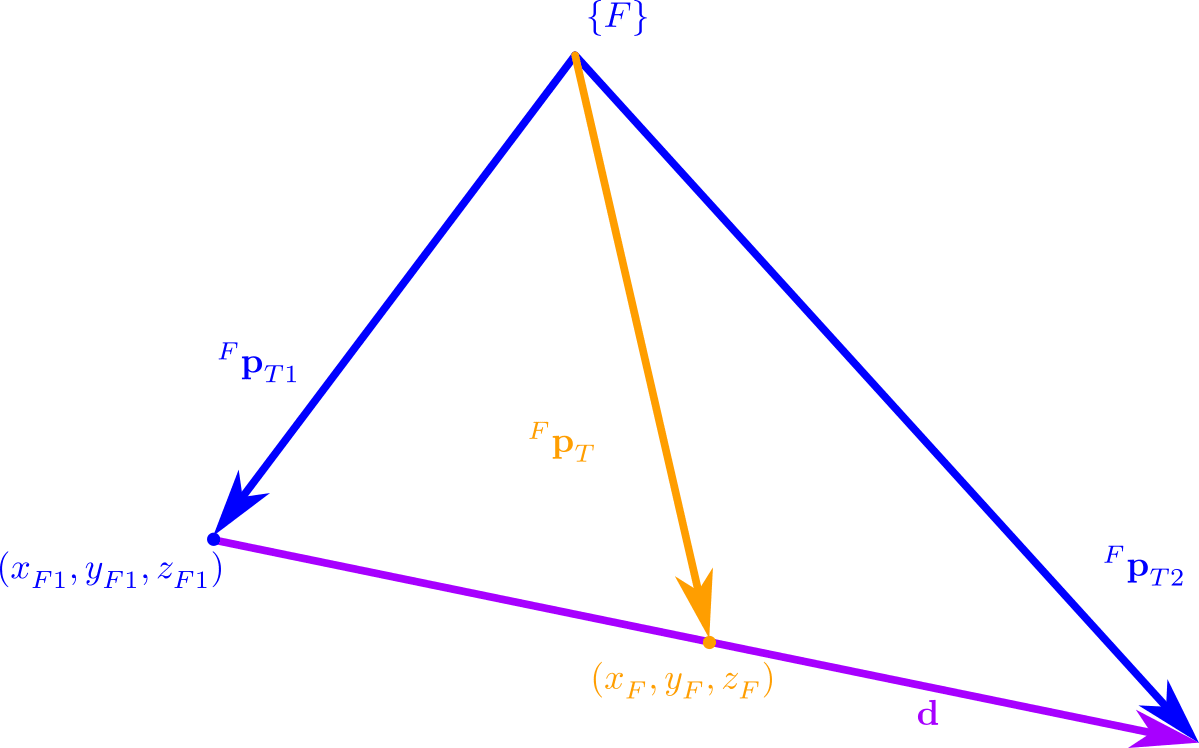
\includegraphics[width=10cm]{images/line-segment-trajectory-wrt-fulcrum.png}\\
\caption{Line segment trajectory of tool tip with respect to Fulcrum reference frame}
\end{figure}
\end{center}
\[
\mathbf{d} = {}^{F}\mathbf{p}^{}_{T2} - {}^{F}\mathbf{p}^{}_{T1} = [l, m, n]^\top
\]
\[
{}^{F}\mathbf{p}^{}_{T} = [x^{}_{F}, y^{}_{F}, z^{}_{F}]^\top
\]
\[
{}^{F}\mathbf{p}^{}_{T} = {}^{F}\mathbf{p}^{}_{T1} + t\mathbf{d}
\]
\[
t = \frac{x^{}_{F} - x^{}_{F1}}{l} = \frac{y^{}_{F} - y^{}_{F1}}{m} = \frac{z^{}_{F} - z^{}_{F1}}{n} \;\; t \in [0, 1]
\]
\[
\begin{cases}
x^{}_{F} = tl + x^{}_{F1} \\
y^{}_{F} = tm + y^{}_{F1} \\
z^{}_{F} = tn + z^{}_{F1}
\end{cases}
\]
After having calculated the cartesian coordinates we can calculate the spherical coordinates using the \ref{eqns:cartesian-to-spherical} equations.

The line segment trajectory of tool tip, as analysed in this section needs no implementation as 
it is already implemented in the ROS MoveIt library and can be used by calling the method 
\textbf{computeCartesianPath}.

\subsection{Task space analysis}

Dexterity analysis for tool's task space
\begin{equation}
\mathcal{D} = \mathcal{L}_q \mathcal{M}
\end{equation}
where
\begin{equation}
\mathcal{M} = \sqrt{det(J J^\top)}
\end{equation}
\begin{equation}
\mathcal{L}_{q}=1-\exp\left\{-\kappa\prod_{i=1}^{n_{k}}\frac{(q_{ {i}}-q_{i,\min})(q_{i,\max}-q_{i})}{(q_{i,\max}-q_{i,\min})^{2}}\right\}
\end{equation}

\begin{center}
\begin{figure}[H]
\centering
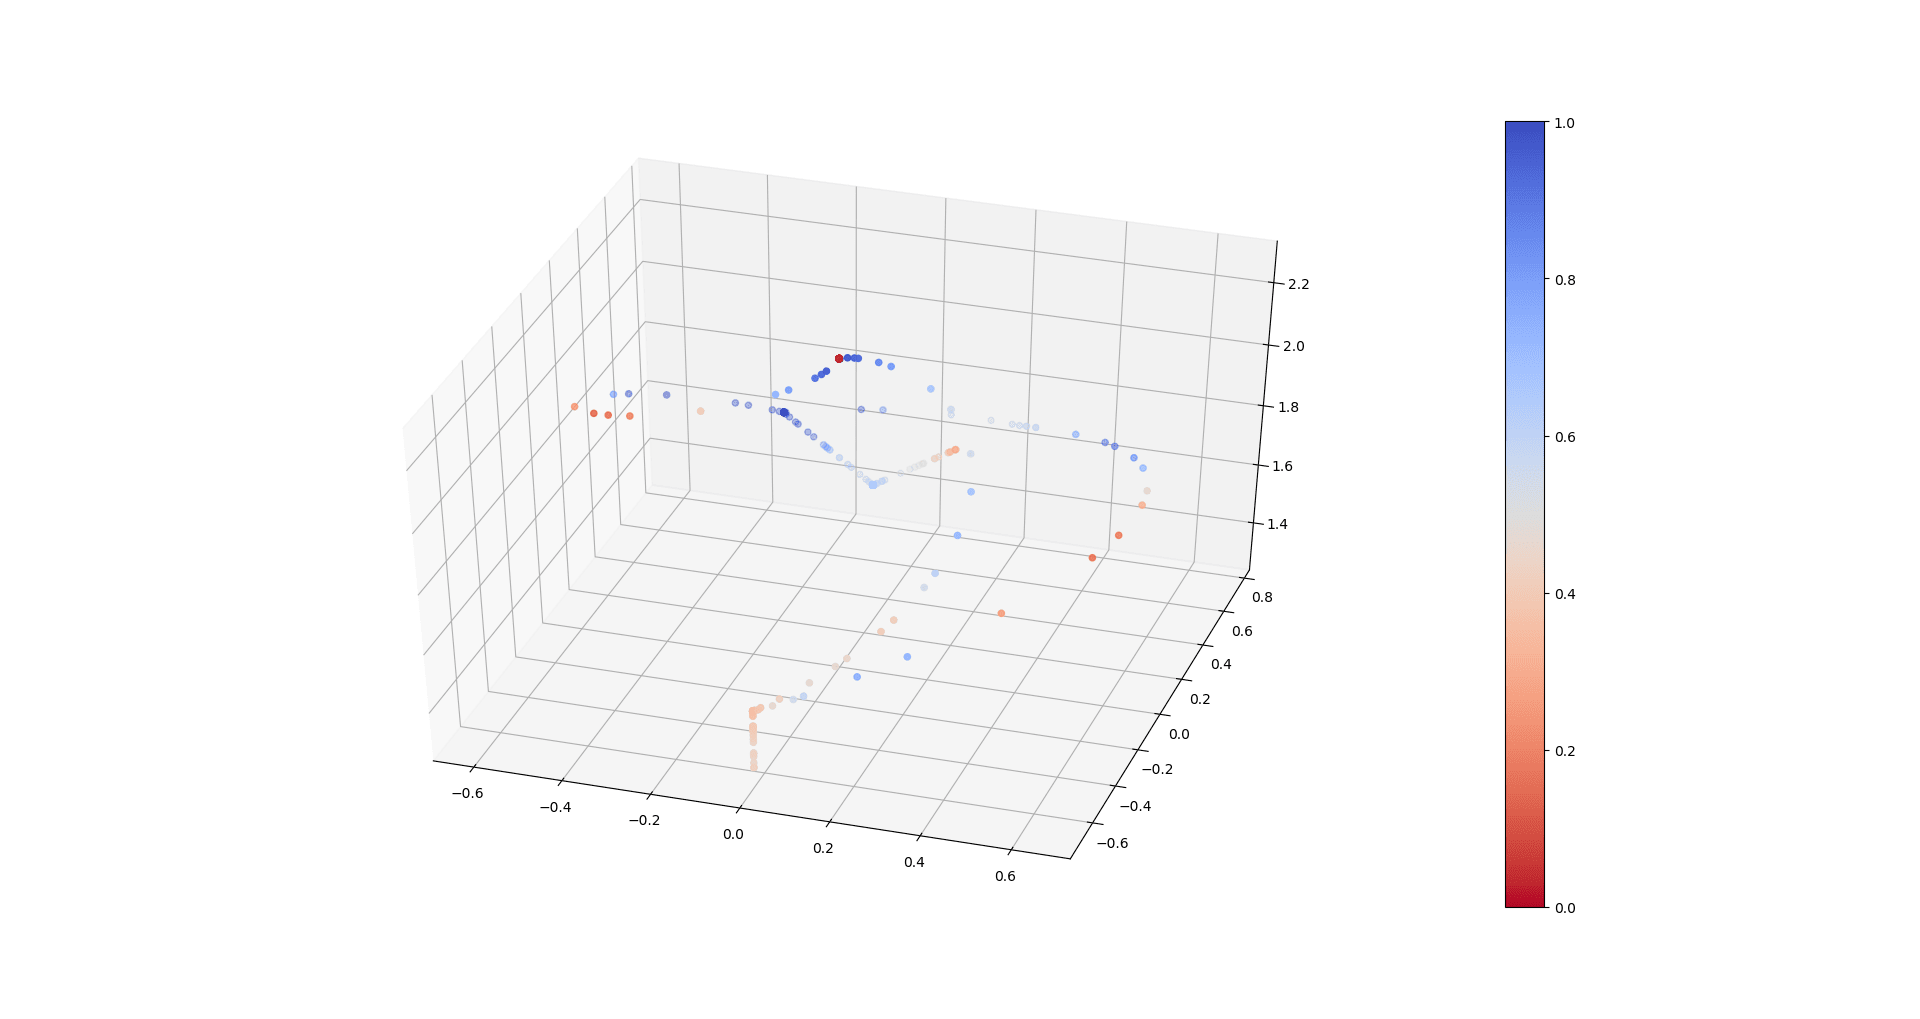
\includegraphics[width=10cm]{images/robot-planner1-manipulability-plot.png}\\
\caption{Plot the manipulability of the robot arm at sample points of the executed trajectory}
\end{figure}
\end{center}

For maximum dexterity at most points of a trajectory in a pivoting motion, the pivot sub-
taskspace (i.e. the space of all configurations of feasible pivot motions) must be fully within 
the robot’s whole reachable taskspace, otherwise only a small range of pivot movements will be 
feasible.